\documentclass[journal]{IEEEtran}
\usepackage[a5paper, margin=10mm]{geometry}
%\usepackage{lmodern} % Ensure lmodern is loaded for pdflatex
\usepackage{tfrupee} % Include tfrupee package

%iffalse
\let\negmedspace\undefined
\let\negthickspace\undefined
\usepackage{gvv-book}
\usepackage{gvv}
\usepackage{cite}
\usepackage{amsmath,amssymb,amsfonts,amsthm}
\usepackage{algorithmic}
\usepackage{graphicx}
\usepackage{textcomp}
\usepackage{xcolor}
\usepackage{txfonts}
\usepackage{listings}
\usepackage{enumitem}
\usepackage{mathtools}
\usepackage{gensymb}
\usepackage{comment}
\usepackage[breaklinks=true]{hyperref}
\usepackage{tkz-euclide} 
\usepackage{listings}                                        
%\def\inputGnumericTable{}                                 
\usepackage[latin1]{inputenc}                                
\usepackage{color}                                            
\usepackage{array}                                            
\usepackage{longtable}                                       
\usepackage{calc}                                             
\usepackage{multirow}                                         
\usepackage{hhline}                                           
\usepackage{ifthen}                                           
\usepackage{lscape}
\usepackage{tabularx}
\usepackage{array}
\usepackage{float}
\usepackage{multicol}

\newcommand{\BEQA}{\begin{eqnarray}}
\newcommand{\EEQA}{\end{eqnarray}}
%\newcommand{\define}{\stackrel{\triangle}{=}}

\setlength{\headheight}{1cm} % Set the height of the header box
\setlength{\headsep}{0mm}     % Set the distance between the header box and the top of the text


%\usepackage[a5paper, top=10mm, bottom=10mm, left=10mm, right=10mm]{geometry}


\setlength{\intextsep}{10pt} % Space between text and floats

% Marks the beginning of the document
\begin{document}
\onecolumn
\bibliographystyle{IEEEtran}
\vspace{3cm}

%\renewcommand{\theequation}{\theenumi}
\numberwithin{equation}{enumi}
\numberwithin{figure}{enumi}
\renewcommand{\thefigure}{\theenumi}
\renewcommand{\thetable}{\theenumi}

\title{Matgeo - 1-1.2-19}
\author{AI24BTECH11030 - Shiven Bajpai}
\maketitle

\textbf{Question: } Find the slope of lines\\
\begin{enumerate}
	\item{Passing through the points \brak{3, -2} and \brak{-1, 4}}
	\item{Passing through the points \brak{3, -2} and \brak{7, -2}}
	\item{Passing through the points \brak{3, -2} and \brak{3, 4}}
	\item{Making inclination of $60\degree$ with the positive direction of x-axis.}
\end{enumerate}

\textbf{Solution: }\\
\begin{enumerate}
	\item{
			\begin{align} m = B-A &= \myvec{3 \\ -2} - \myvec{-1 \\ 4} \\
				&= \myvec{4 \\ -6} \\
				&= 4\myvec{1 \\ \frac{-3}{2}}
		\end{align}
		$\therefore \text{slope is } \frac{3}{2}$
	}
	\item{
			\begin{align} m = B-A &= \myvec{3 \\ -2} - \myvec{7 \\ -2} \\
				&= \myvec{-4 \\ 0} \\
				&= -4\myvec{1 \\ 0}
		\end{align}
		$\therefore \text{slope is } 0$
	}
	\item{
			\begin{align} m = B-A &= \myvec{3 \\ -2} - \myvec{3 \\ 4} \\
				&= \myvec{0 \\ -6} \\
				&= 6\myvec{0 \\ -1}
		\end{align}
		$\therefore \text{slope is } -\infty$
	}
	\item{
			\begin{align} m &= \myvec{\cos \alpha \\ \sin \alpha} \\
				&= \myvec{\cos 60\degree \\ \sin 60\degree} \\
				&= \myvec{\frac{1}{2} \\ \frac{\sqrt{3}}{2}} \\
				&= \frac{1}{2} \myvec{1 \\ \sqrt{3}}
		\end{align}
		$\therefore \text{slope is } \sqrt{3}$
	}
\end{enumerate}

\begin{figure}[H]
	\centering
	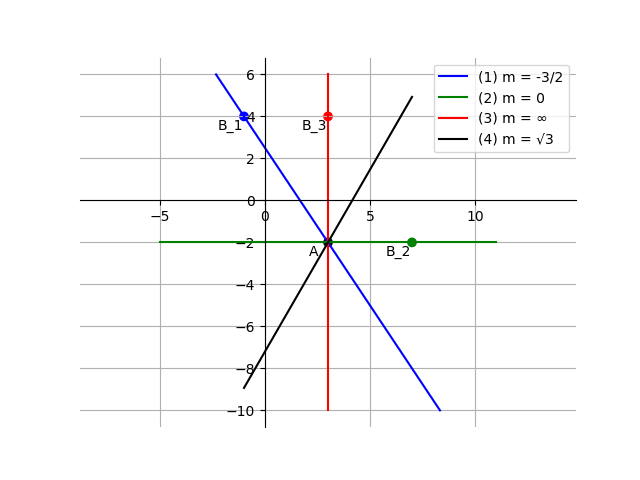
\includegraphics[width=0.75\columnwidth]{Figures/Figure.png}
	\caption{A plot of all lines}
	\label{fig}
\end{figure}

Code for plotting points and vector arithmetic
\begin{lstlisting}
	Codes/linear.py
\end{lstlisting}

\renewcommand{\thefigure}{\theenumi}
\renewcommand{\thetable}{\theenumi}


\end{document}
